
\section{Experimental Analysis}\label{sec:exp}
These benchmarks were carried out on a Razer Blade Pro laptop with Intel Core i7-10875H CPU @ 2.30GHz (Max 5.10 GHz) (8 Cores 16 Logical Processors), 16GB DDR4 2933MHz RAM and 315GB free disk space.
\begin{figure}[!t]
	\centering
	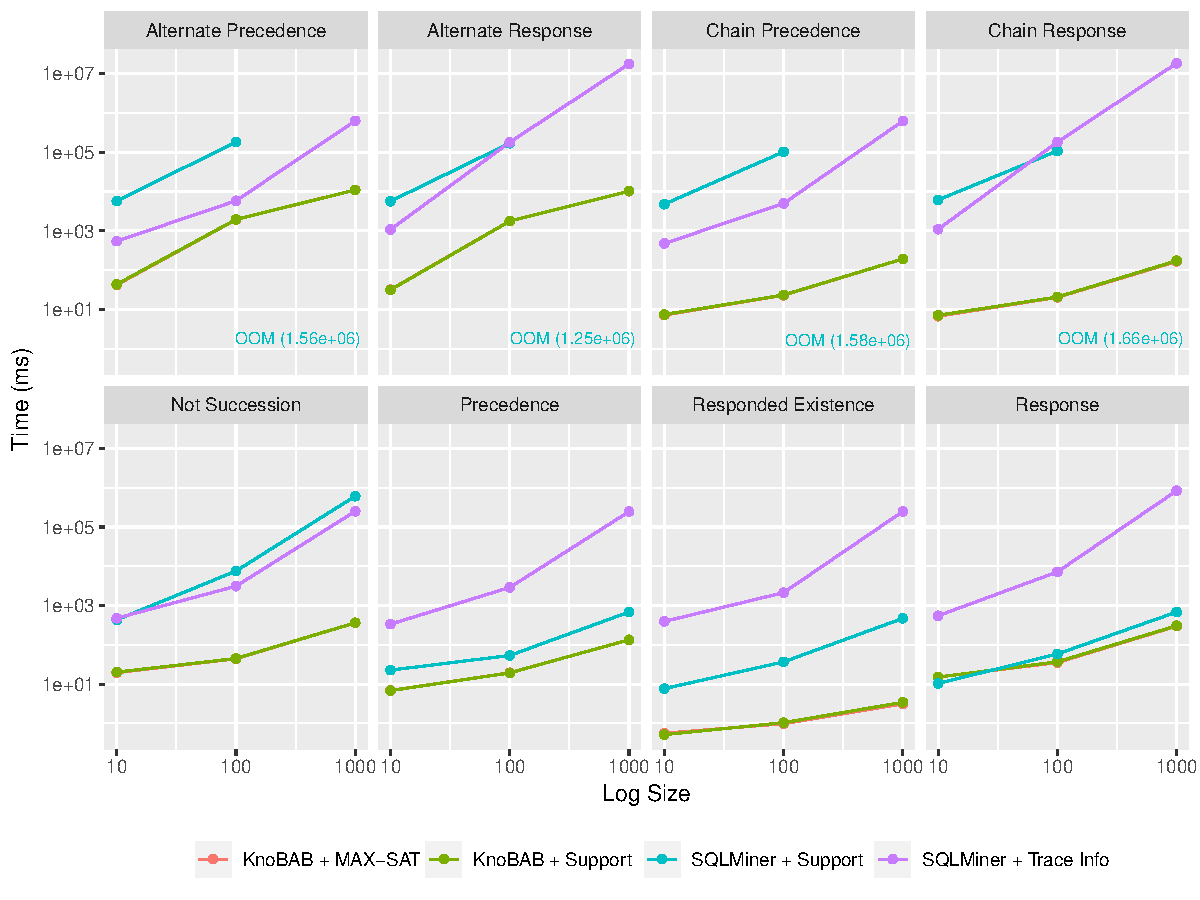
\includegraphics[width=.8\textwidth]{images/sqlminer_benchmark.pdf}
	\caption{KnoBAB vs SQLMiner Performance for 25  clauses with frequent activity labels with Support and Trace Information. OOM indicates Out of Memory, where $>$ 315GB of secondary memory was used (causing memory failure).}\label{fig:vsSQL}
\end{figure}

\subsection{SQLMiner}\label{ssec:sqlmin}

\textbf{PostgreSQL 13.5}  (\figurename~\ref{fig:vsSQL})


\begin{table}[!t]
	\caption{Satisfiability over the BPI 2012 Challenge}
	\centering
	\resizebox{\textwidth}{!}{\begin{tabular}{l|r|rr}
			\toprule
			\multirow{2}{*}{\textit{Conjunctive Query}} & \multicolumn{3}{c}{Query Time \textit{(ms)}} \\ 
			& \textsf{Declare Analyzer} & \textbf{KnoBAB+Conj}& \textbf{KnoBAB+Supp}\\
			\midrule
			$q_1:= \DeclareClause{Response}{A\_SUBMITTED}{\textbf{true}}{A\_ACCEPTED}{\textbf{true}}$ &  $\color{red}1.75\cdot 10^3$ & $\mathbf{1.83}\cdot \mathbf{10}^\mathbf{1}$& $2.19\cdot 10^1$\\
			$q_2:= q_1\wedge \MonoDeclareClause{Exists}{\_\_trace\_payload}{\texttt{AMOUNT\_REQ}\geq 10^3}{\geq 1}$ &  $\color{red}1.77\cdot 10^3$ & $\mathbf{2.06}\cdot \mathbf{10}^\mathbf{1}$ & $2.45\cdot 10^1$ \\
			$q_3:=q_1\wedge \MonoDeclareClause{Exists}{\_\_trace\_payload}{\texttt{AMOUNT\_REQ}< 10^3}{\geq 1}$ & $\color{red}1.62\cdot 10^3$ & $\mathbf{2.15}\cdot \mathbf{10}^\mathbf{1}$&  $2.51\cdot 10^1$\\
			$q_4:=q_1\textrm{ where }\texttt{A\_SUBMITTED.org:resource}=\texttt{A\_ACCEPTED.org:resource}$ & $\color{red}1.71\cdot 10^3$ & $\mathbf{2.43}\cdot \mathbf{10}^\mathbf{1}$& $2.77\cdot 10^1$\\
			$q_5:=q_1\textrm{ where }\texttt{A\_SUBMITTED.org:resource}\neq\texttt{A\_ACCEPTED.org:resource}$ & $\color{red}1.93\cdot 10^3$ & $\mathbf{2.59}\cdot \mathbf{10}^\mathbf{1}$& $3.01\cdot 10^1$\\
			$q_1\wedge q_2$ & $\color{red}1.81\cdot 10^3$ &  $\mathbf{2.70}\cdot \mathbf{10}^\mathbf{1}$& $3.05\cdot 10^1$\\
			$q_1\wedge q_2\wedge q_4$ & $\color{red}2.49\cdot 10^3$ & $\mathbf{2.74}\cdot \mathbf{10}^\mathbf{1}$ & $3.15\cdot 10^1$\\
			$q_1\wedge q_3\wedge q_4$ & $\color{red}2.38\cdot 10^3$ & $\mathbf{2.51}\cdot \mathbf{10}^\mathbf{1}$& $2.80\cdot 10^1$\\
			$q_1\wedge q_2\wedge q_5$ &$\color{red}2.06\cdot 10^3$  & $\mathbf{2.57}\cdot \mathbf{10}^\mathbf{1}$& $2.95\cdot 10^1$\\
			$q_1\wedge q_3\wedge q_5$ & $\color{red}2.19\cdot 10^3$ & $\mathbf{2.29}\cdot \mathbf{10}^\mathbf{1}$& $2.55\cdot 10^1$\\
			$q_1\wedge q_2\wedge q_3\wedge q_4\wedge q_5$ & $\color{red}2.90\cdot10^3$ & $\mathbf{2.66}\cdot \mathbf{10}^\mathbf{1}$ & $3.01\cdot 10^1$\\
			\bottomrule
	\end{tabular}}
\end{table}

\subsection{Declare Analyzer}\label{ssec:declan}

The benefits from the custom query plan are most obvious in the process mining stage, where a log consisting of potentially thousands of traces is tested against all combinations of clauses. However, computational gains can also be evidenced when the same querying approach is adapted to a runtime scenario, where we are querying only 1 trace against an existing model (which requires much less computation as a whole).

For $\mathcal{C}$ Declare clauses, where $\mathcal{N}$ is the data loading cost, implementations without a KB suffer, resulting in $\mathcal{O(C \cdot N)}$ complexity. With a KB, data loading is necessary only once, enhancing the complexity to $\mathcal{O(C + N)}$.

However these are computationally bottlenecked to the efficiency of these systems themselves, regardless of the optimality of the conformance checking.

\RevDel{SQL miner, due to the query structure, requires vast amounts of secondary memory for temporary caching of query computation, {much less than KnoBAB requires}.}